\documentclass[12pt]{report}
\usepackage[margin=1in]{geometry}
\usepackage{hyperref}
\usepackage{url}
\usepackage{xurl}
\hypersetup{breaklinks=true}
\usepackage{graphicx}
\usepackage{amsmath}
\usepackage{enumitem}
\usepackage{float}

\title{Week 7 Report}
\author{Dhanush Balusa}
\date{July 2nd, 2025}

\begin{document}

\maketitle

\chapter*{Research}

\noindent \textbf{Gabbard Diagram: }
\begin{itemize}
  \item Gabbard Diagram Formation: The General Theory for Elliptical Orbits: \url{https://www.ripublication.com/aasa18/aasav8n2_01.pdf}
  \item A Gabbard diagram plots the apogee and perigee heights of the space debris vs. the orbital periods of the space debris.
  \item Gabbard diagrams help in understanding the nature of the orbit, the fragmentation point, and the spread of fragments.
\end{itemize}

\noindent \textbf{Conjunction analysis:}
\begin{enumerate}

  \item Spaceflight Safety Handbook For Satellite Operators: \url{https://for-testing-only.space-track.org/documents/SFS_Handbook_For_Operators_V1.7.pdf}

  \begin{itemize}
    \item Uses Special Perturbations (SP) orbit propagation theory.
    \item SP includes high-accuracy modeling of gravitational and non-gravitational forces, enabling reliable propagation of Resident Space Objects (RSOs).
    \item Propagation uses data from the Space Surveillance Network (SSN) sensors worldwide. This data feeds into the High Accuracy Catalog (HAC), which is updated every 8 hours.
    \item Other parameters that are important in conjunction analysis include:
    \begin{itemize}
      \item Covariance Matrices: Quantify uncertainty in an object's position and velocity.
      \item Predictive Ephemerides: Submitted by operators in formats like OEM. Predictive ephemerides are time-stamped position/velocity trajectories submitted by satellite operators, describing where their spacecraft will be in the future. These inputs allow 19 SDS to predict conjunctions involving future maneuvers and provide decision support to operators on whether an avoidance action is necessary.
      \item Maneuver Intent: Operators must report maneuvers; otherwise, risk assessments may be inaccurate.
    \end{itemize}
  \end{itemize}

   \item NASA Spacecraft Conjunction Assessment and Collision Avoidance Best Practices Handbook: \url{https://nodis3.gsfc.nasa.gov/OCE_docs/OCE_51.pdf}

  \begin{itemize}
    \item NASA advises against using TLEs, which rely on the SGP4 model, because TLEs do not include covariances and are too imprecise for collision probability calculation.
    \item Other parameters that are important in conjunction analysis include:
    \begin{itemize}
      \item Predictive Ephemerides: NASA uses Orbit Ephemeris Message (OEM)-formatted data with covariances, including maneuvers. Delivered via space-track.org and NASA’s internal channels.
      \item Force Models Used: Drag, solar radiation pressure, and third-body perturbations are used in conjunction analysis.
      \item Probability of Collision (Pc) Calculations: NASA uses 2D Pc, 3D Number of Collisions (Nc), and Monte Carlo methods.
      \item Relative Geometry at TCA: TCA risk is evaluated using radial, in-track, and cross-track miss distances.
    \end{itemize}
  \end{itemize}

\end{enumerate}

\chapter*{Code Changes}

To clean up the code and based on the feedback from Space-Track.org, I decided to make the following changes:

\begin{enumerate}
  
  \item \textbf{My first change was to implement my plan of action to ensure that the code is compliant with Space-Track’s API rules.}
  
    The TLE fetching script has been updated to follow the Space-Track.org API rules.

    \begin{figure}[H]
      \centering
      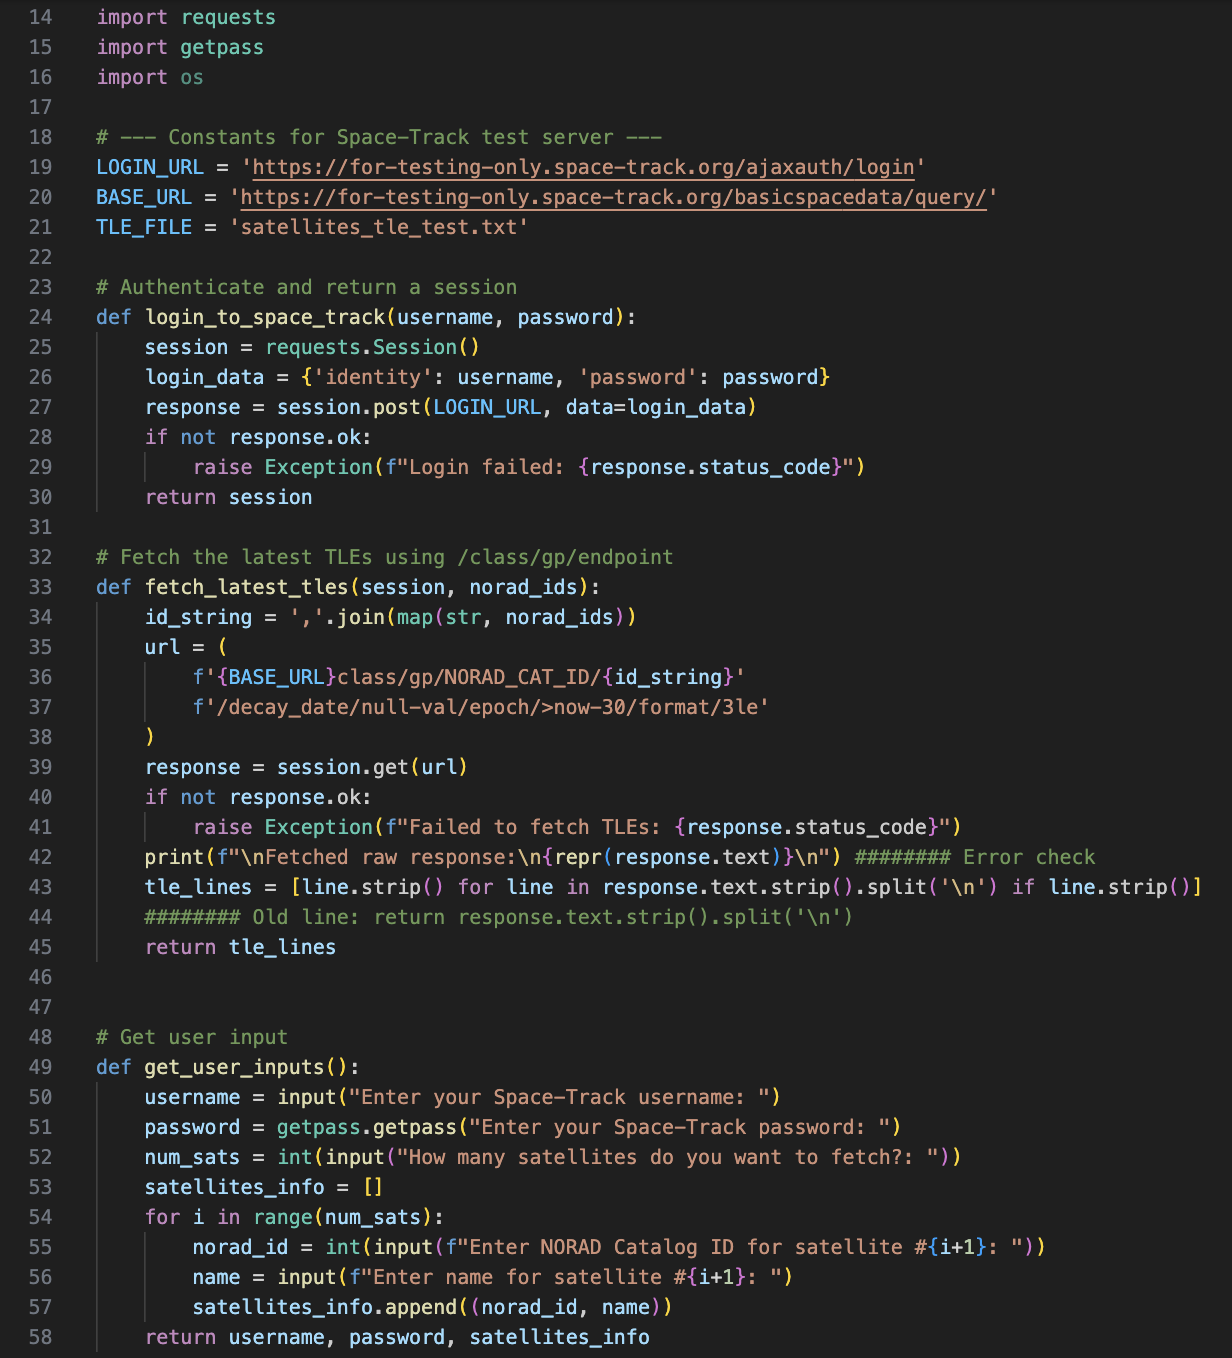
\includegraphics[width=0.8\textwidth]{figure_week_7_fetch1.png}
      \caption{Script for fetching TLE data from Space-Track.org.}
      \label{fig:fetch-tle-data1}
    \end{figure}

    \begin{figure}[H]
      \centering
      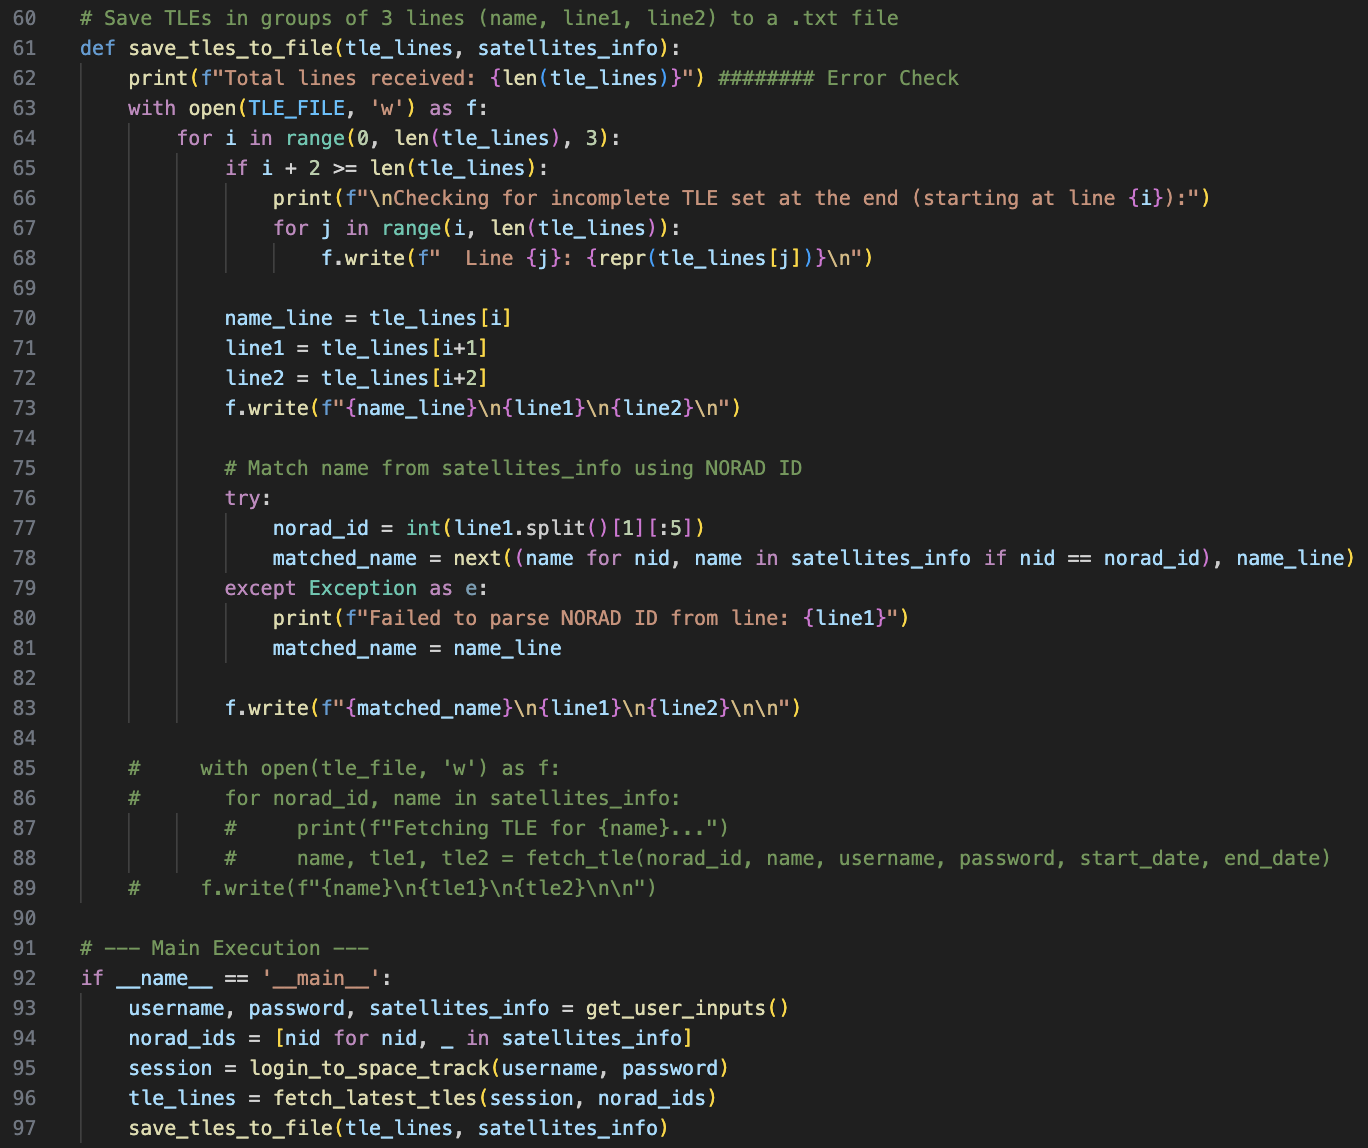
\includegraphics[width=0.8\textwidth]{figure_week_7_fetch2.png}
      \caption{Script for saving TLE data to a local file.}
      \label{fig:fetch-tle-data2}
    \end{figure}

    I'm having issues with fetching the TLE data from Space-Track.org's test API. I think it's just an issue of TLE formating because I had to change that last time, but I'm not sure. I've created a lot of new functions this time, but only \texttt{fetch\_latest\_tles} and/or \texttt{save\_tles\_to\_file} seem to be the problamatic ones.
    \\ \\
    Here is the output that I am getting:

    \begin{figure}[H]
      \centering
      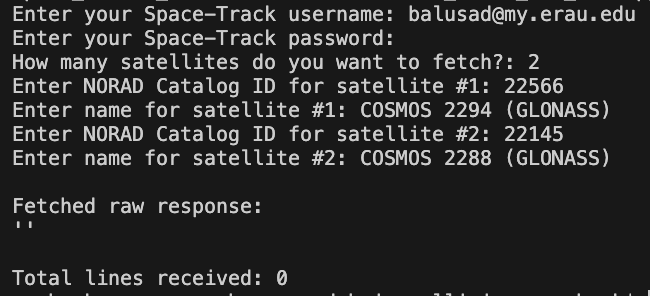
\includegraphics[width=0.8\textwidth]{figure_week_7_fetch-output.png}
      \caption{Output for fetching TLE conditions.}
      \label{fig:fetch-tle-data-out}
    \end{figure}

    The analysis script seems to be working fine based on a fake TLE data file I created and even plots the output. It looks like it's working fine, because there is no logic change in the code.
    \\ \\
    Also, I will only be using this script for historical TLE data analysis because Space-Track's Sync.com archive already provides files of data (per year).

    \begin{figure}[H]
      \centering
      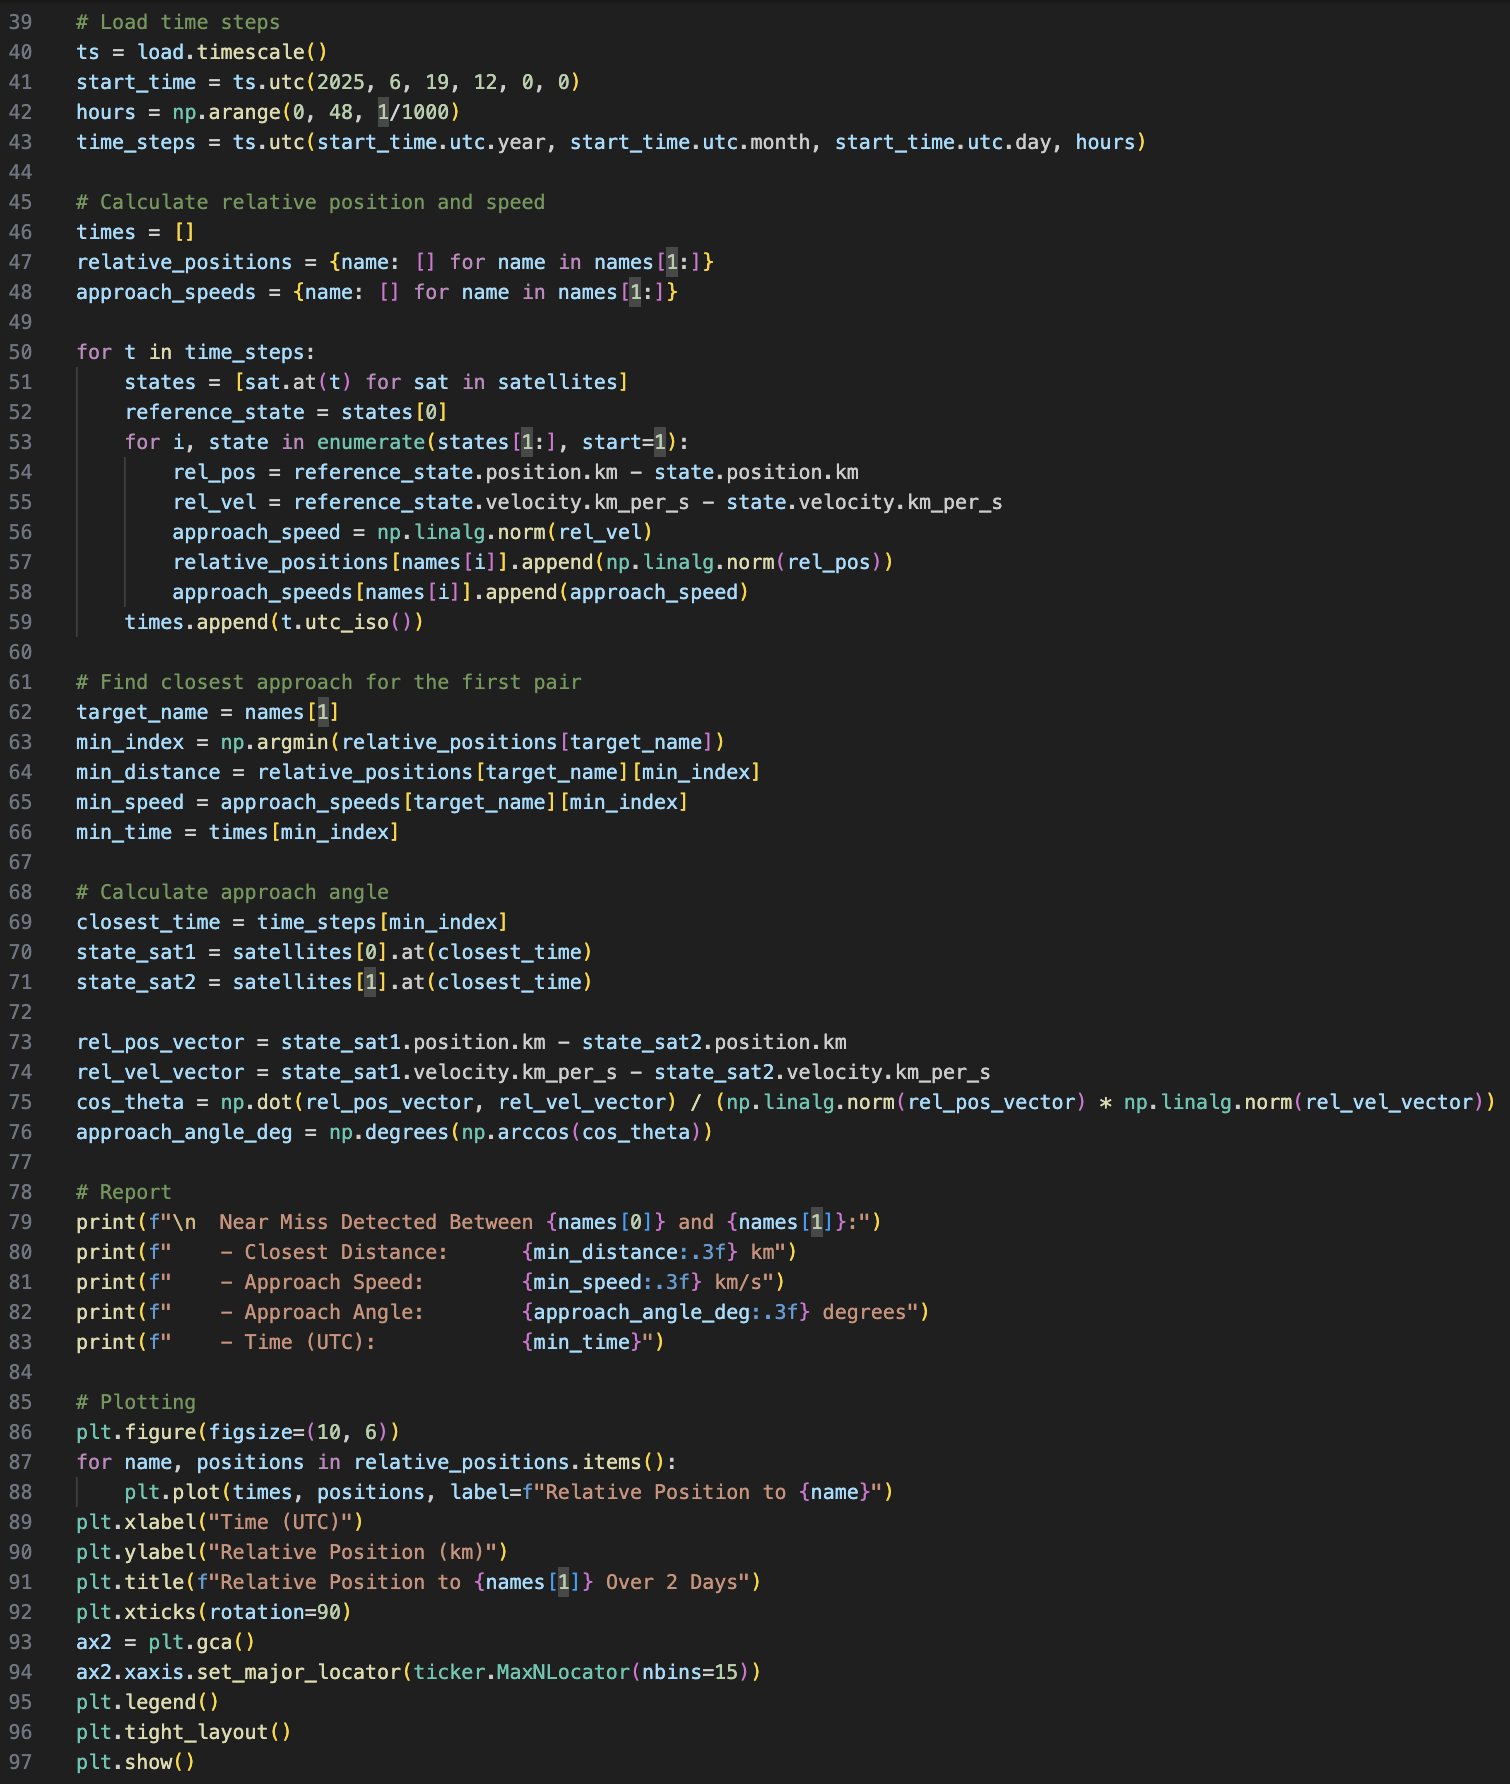
\includegraphics[width=0.8\textwidth]{figure_week_6_analyze-approach.png}
      \caption{Script for analyzing approach conditions.}
      \label{fig:analyze-tle-data}
    \end{figure}

    \begin{figure}[H]
      \centering
      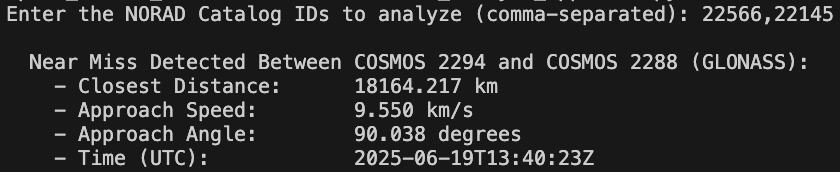
\includegraphics[width=0.8\textwidth]{figure_week_7_analysis-output.png}
      \caption{Input and output for for analyzing approach conditions.}
      \label{fig:analyze-tle-data-out}
    \end{figure}
  
  \item \textbf{My second change was to check if I find the spacecraft type (i.e. debris, rocket body, operational satellite) from the TLE data? If it's possible, I will plot data points coresponding to each spacecraft type (by color).}
  
  Because I was not successful in fetching the TLE data from Space-Track.org's test API, I can not surely tell. If the API provides the spacecraft name, I can try to find the spacecraft type from the name. For example, if the name contains "DEB" or "R/B", I can classify it as debris or rocket body, respectively. However, this is not a foolproof method and may not work for all cases.

\end{enumerate}

\chapter*{Next Steps}

\textbf{My Next Steps:}
\begin{itemize}
  \item Debug the \texttt{fetch\_latest\_tles} and \texttt{save\_tles\_to\_file} functions to ensure they function correctly. The \texttt{save\_tles\_to\_file} function is where the code fails, especially test case \texttt{if\ i\ +\ 2\ >=\ len(tle\_lines)}.
  \item Test the new scripts to ensure they work as expected and fetch the latest TLE data correctly. Use the 4 test cases from Week 5 to verify.
  \item Plot the data points coresponding to each spacecraft type (by color).
\end{itemize}

\noindent \textbf{Dr. Fan's feedback for next steps:}
\begin{enumerate}
  \item Read into orbit covariance, either covariance of orbital elements or states (position \& velocity).
  \item How to propogate covariance, analytically or numerically (Monte Carlo or sigma points).
  \item How to identify collision when there is covariance information.
  \item Orbit propagator using: two-body, oblateness (J2), third body (moon), drag (if possible).
\end{enumerate}

\noindent \textbf{End goals:}
\begin{itemize}
  \item Loop through all the TLEs in the different categories and calculate the approach conditions for each satellite if it is within a certain distance (e.g. 100 km) of the ISS.
  \item Incorporate covariance into space object propagation for more realistic collision identification. Also for warning time first propogate for 7 days. 
  \item Make my code a usable function so Catherine can just call it. Some input \textrightarrow{} Output (approach speed and angle).
\end{itemize}

\end{document}